\documentclass{standalone}
\usepackage{tikz}
\begin{document}

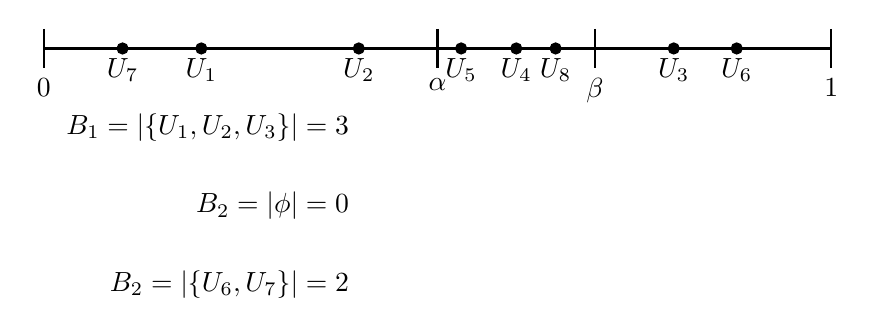
\begin{tikzpicture}

    % Draw the line representing the interval
    \draw[thick] (0,0) -- (10,0);
    
    % Draw the points U1, U2, U4, U3
    \filldraw (2,0) circle (2pt) node[below] {$U_1$};
    \filldraw (4,0) circle (2pt) node[below] {$U_2$};
    \filldraw (6,0) circle (2pt) node[below] {$U_4$};
    \filldraw (5.3,0) circle (2pt) node[below] {$U_5$};
    \filldraw (8.8,0) circle (2pt) node[below] {$U_6$};
    \filldraw (8,0) circle (2pt) node[below] {$U_3$};
    \filldraw (1,0) circle (2pt) node[below] {$U_7$};
    \filldraw (6.5,0) circle (2pt) node[below] {$U_8$};
    
    % Mark the intervals (alpha, beta)
    \draw[thick] (0,0.25) -- (0,-0.25) node[below] {$0$};
    \draw[thick] (5,0.25) -- (5,-0.25) node[below] {$\alpha$};
    \draw[thick] (7,0.25) -- (7,-0.25) node[below] {$\beta$};
    \draw[thick] (10,0.25) -- (10,-0.25) node[below] {$1$};

    % % Draw the gaps L1, L2, L3
    % \draw[<->] (0,0.5) -- (2,0.5) node[midway, above] {$L_1$};
    % \draw[<->] (0,1) -- (4,1) node[midway, above] {$L_2$};
    % \draw[<->] (0,1.5) -- (8,1.5) node[midway, above] {$L_3$};

    % Add labels for the geometric distribution
    \node[left] at (4,-1) {$B_1=|\{U_1,U_2,U_3\}|=3$};
    \node[left] at (4,-2) {$B_2=|\phi|=0$};
    \node[left] at (4,-3) {$B_2=|\{U_6,U_7\}|=2$};

\end{tikzpicture}

\end{document}
